% Overleaf: Menu -> Settings -> Compiler = XeLaTeX -> Recompile
% Upload: main.tex (this file) + figures/ folder

\documentclass[11pt,a4paper]{article}

\usepackage{fontspec}
\setmainfont{Times New Roman}
\usepackage[english]{babel}
\usepackage[a4paper,margin=2cm]{geometry}
\usepackage{graphicx}
\usepackage{booktabs}
\usepackage{hyperref}
\usepackage{enumitem}
\usepackage{listings}
\usepackage{xcolor}
\usepackage{subcaption}

\hypersetup{colorlinks=true, linkcolor=black, urlcolor=blue}
\setlist{nosep, leftmargin=*}
\graphicspath{{figures/}}

\lstset{
  basicstyle=\ttfamily\footnotesize,
  breaklines=true,
  frame=single,
  backgroundcolor=\color{gray!8},
}

\title{\textbf{JournalAI — PRM393 Lab 2}\\[4pt]
\large Source Code Structure, Implementation Techniques, and User Interface}
\author{Tran Nhat Duy (K18 HCM) \\ PRM393\_Lab2\_SE182125}
\date{June 2026}

\begin{document}
\maketitle
\thispagestyle{empty}
\vspace{-0.8em}
\begin{center}
\textit{Source repository: \url{https://github.com/DUUY69/PRM_Lab2}} \quad|\quad
\textit{Flutter · OpenAlex · Provider · fl\_chart}
\end{center}
\vspace{0.8em}

\tableofcontents
\newpage

\section{Project Overview}

\textbf{Journal Trend Analyzer (JournalAI)} is a mobile application for querying and analyzing academic research trends via the \textbf{OpenAlex API}. All data is fetched dynamically from the web service; no static data is embedded in the source code.

The application is organized into three functional tabs: \textbf{Overview}, \textbf{Explore}, and \textbf{About}.

\textbf{Illustrative workflow:} Splash screen $\rightarrow$ Overview $\rightarrow$ Explore (search topic ``ras'') $\rightarrow$ trend chart $\rightarrow$ publication detail.

\section{Source Code Architecture}

\subsection{Three-Layer Model}
\begin{center}
\begin{tabular}{@{}ll@{}}
\toprule
\textbf{Layer} & \textbf{Responsibility} \\
\midrule
\texttt{screens/}, \texttt{widgets/} & User interface — rendering and navigation \\
\texttt{providers/} & State management — \texttt{PublicationProvider} \\
\texttt{services/}, \texttt{models/} & HTTP communication with OpenAlex, JSON mapping \\
\texttt{utils/} & Analytical metrics (growth rate, momentum) \\
\bottomrule
\end{tabular}
\end{center}

\textbf{Data flow:} Screen $\rightarrow$ Provider $\rightarrow$ OpenAlexService $\rightarrow$ Model.

\subsection{Main Directory Tree (\texttt{lib/})}
\begin{lstlisting}
main.dart
screens/   main_shell, overview, search, detail, growth,
           citation_leaders, journals_analysis, keywords_overview,
           research_leaders, author/journal/domain/year_detail, about
providers/ publication_provider.dart, app_navigation_provider.dart
services/  openalex_service.dart, openalex_config.dart
widgets/   trend_chart, keyword_bar_chart, journal_bar_chart,
           topic_trend_analytics, publication_card
models/    publication.dart, openalex_ranked_entity.dart
\end{lstlisting}

\section{Technologies Used}

\begin{tabular}{@{}p{3.2cm}p{10.8cm}@{}}
\toprule
\textbf{Technology} & \textbf{Description} \\
\midrule
Flutter / Provider & UI construction and ChangeNotifier-based state management \\
REST / JSON & API calls via \texttt{http}; data mapping via \texttt{Publication.fromJson} \\
OpenAlex & Queries to \texttt{/works}, grouped by \texttt{group\_by=publication\_year} \\
Asynchronous processing & Future handling, retry on HTTP 503, loading/error states \\
Pagination & 20 records per page on the Explore tab \\
Charts & \texttt{fl\_chart} library: line, pie, and horizontal bar charts \\
SharedPreferences & Persists API key and search history \\
\bottomrule
\end{tabular}

\section{Lab 2 Requirements Mapping}

\begin{tabular}{@{}cll@{}}
\toprule
\textbf{Section} & \textbf{Requirement} & \textbf{Implementation} \\
\midrule
4.1 & Topic search & Explore tab \\
4.2 & Publication detail & \texttt{detail\_screen} \\
4.3 & Trend chart & Explore tab (after search) \\
4.4 & Top-cited papers & Citation Leaders \\
4.5 & Top journals & Publication Sources \\
4.6 & Top authors & Research Leaders \\
4.7 & Overview dashboard & Overview tab \\
\bottomrule
\end{tabular}

\subsection{Charts Implemented per Assignment Specification}
\begin{tabular}{@{}clll@{}}
\toprule
\textbf{No.} & \textbf{Chart Name} & \textbf{Type} & \textbf{Location} \\
\midrule
1 & Publication volume trend & Line chart & Explore, Growth, detail screens \\
2 & Citation trend & Line chart & Citations tab (Explore) \\
3 & Top keywords & Horizontal bar chart & Keyword Overview \\
14 & Journal ranking & Horizontal bar chart & Publication Sources \\
\bottomrule
\end{tabular}

\section{Application Screenshots}

\subsection{Splash Screen}
\begin{figure}[htbp]
  \centering
  
\includegraphics[width=0.36\textwidth]{fig01-splash.jpg}
  \caption{Splash screen — loading data from OpenAlex}
\end{figure}

\subsection{Overview Tab — Dashboard (Section 4.7)}
\begin{figure}[htbp]
  \centering
  \begin{subfigure}{0.48\textwidth}
    \centering
    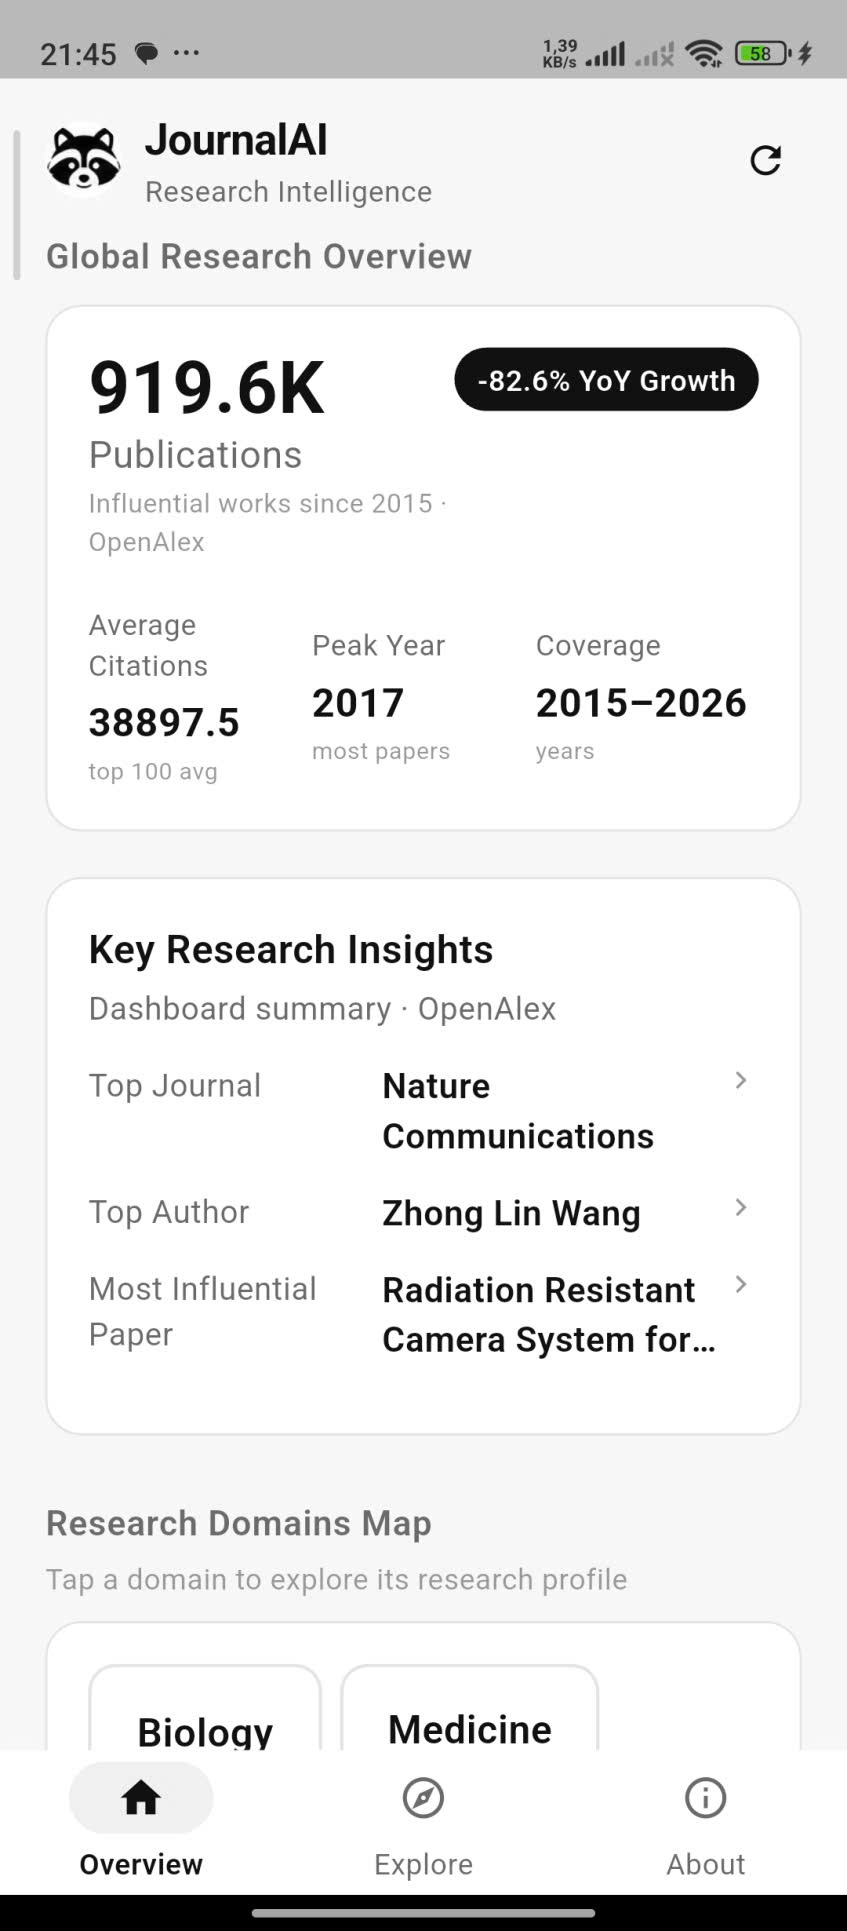
\includegraphics[width=\textwidth]{fig02-overview.jpg}
    \caption{Overview and key research insights}
  \end{subfigure}\hfill
  \begin{subfigure}{0.48\textwidth}
    \centering
    
\includegraphics[width=\textwidth]{fig03-overview-tiles.jpg}
    \caption{Research landscape distribution}
  \end{subfigure}
  \caption{Overview tab interface}
\end{figure}

\subsection{Explore Tab — Search and Trend Analysis (Sections 4.1, 4.3)}
Sample search topic: \textbf{ras}.

\begin{figure}[htbp]
  \centering
  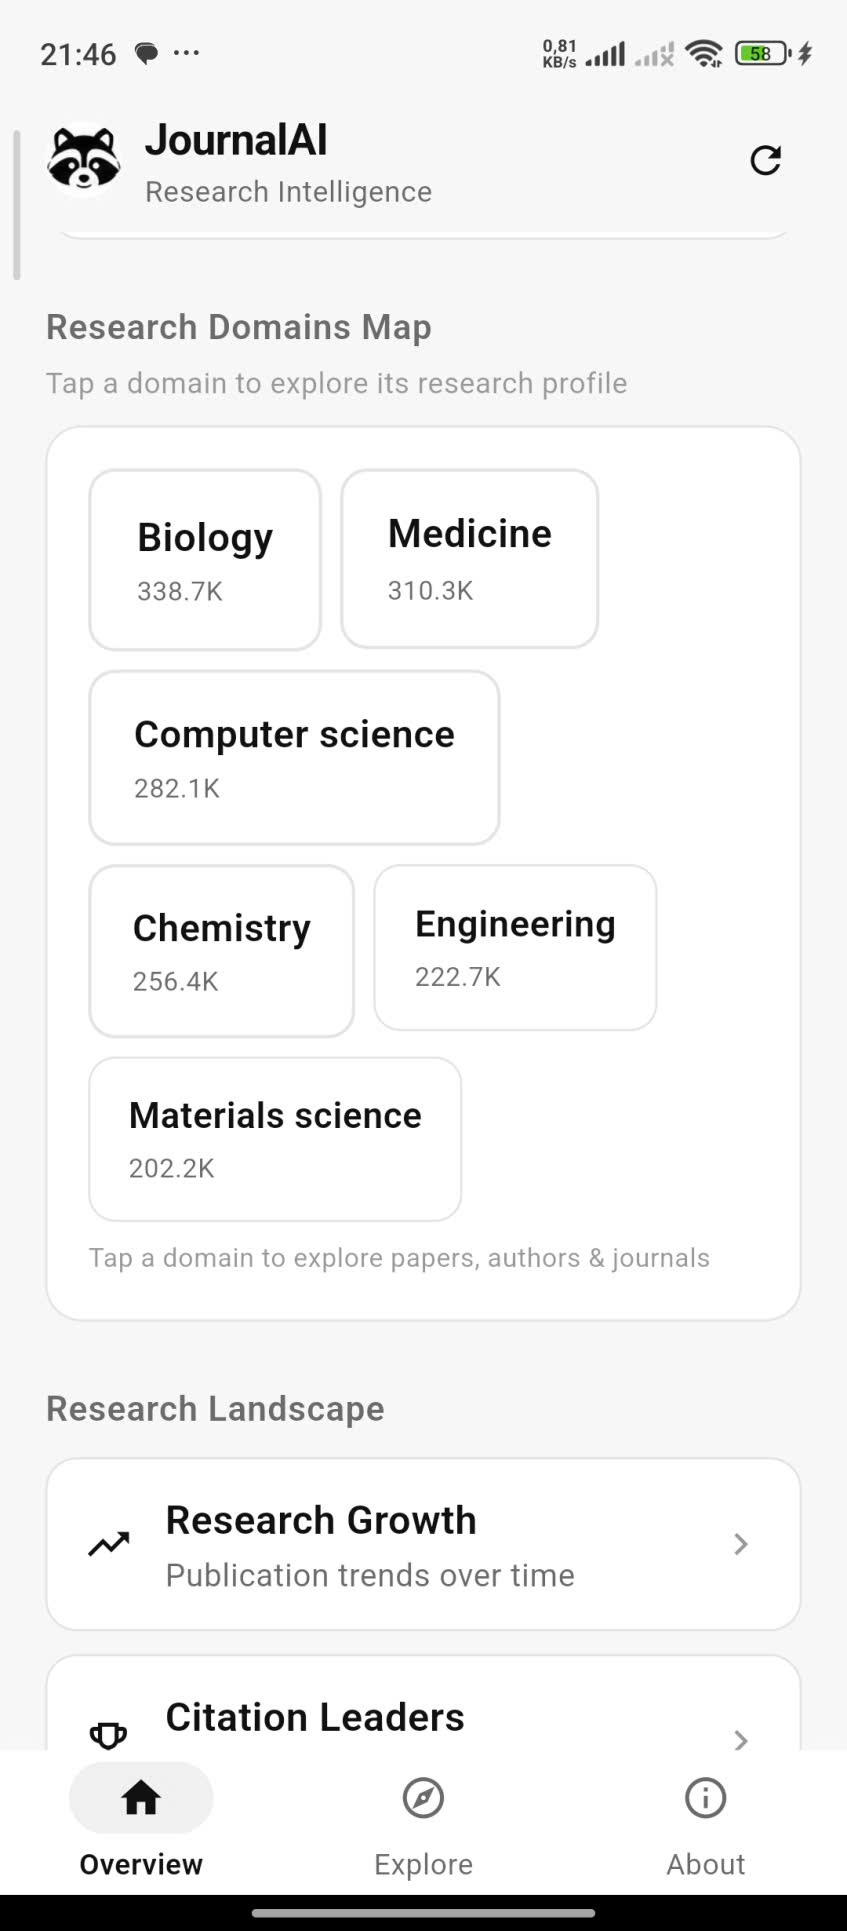
\includegraphics[width=0.42\textwidth]{fig11-explore-topics.jpg}
  \caption{Topic summary with top journals and authors}
\end{figure}

\begin{figure}[htbp]
  \centering
  \begin{subfigure}{0.48\textwidth}
    \centering
    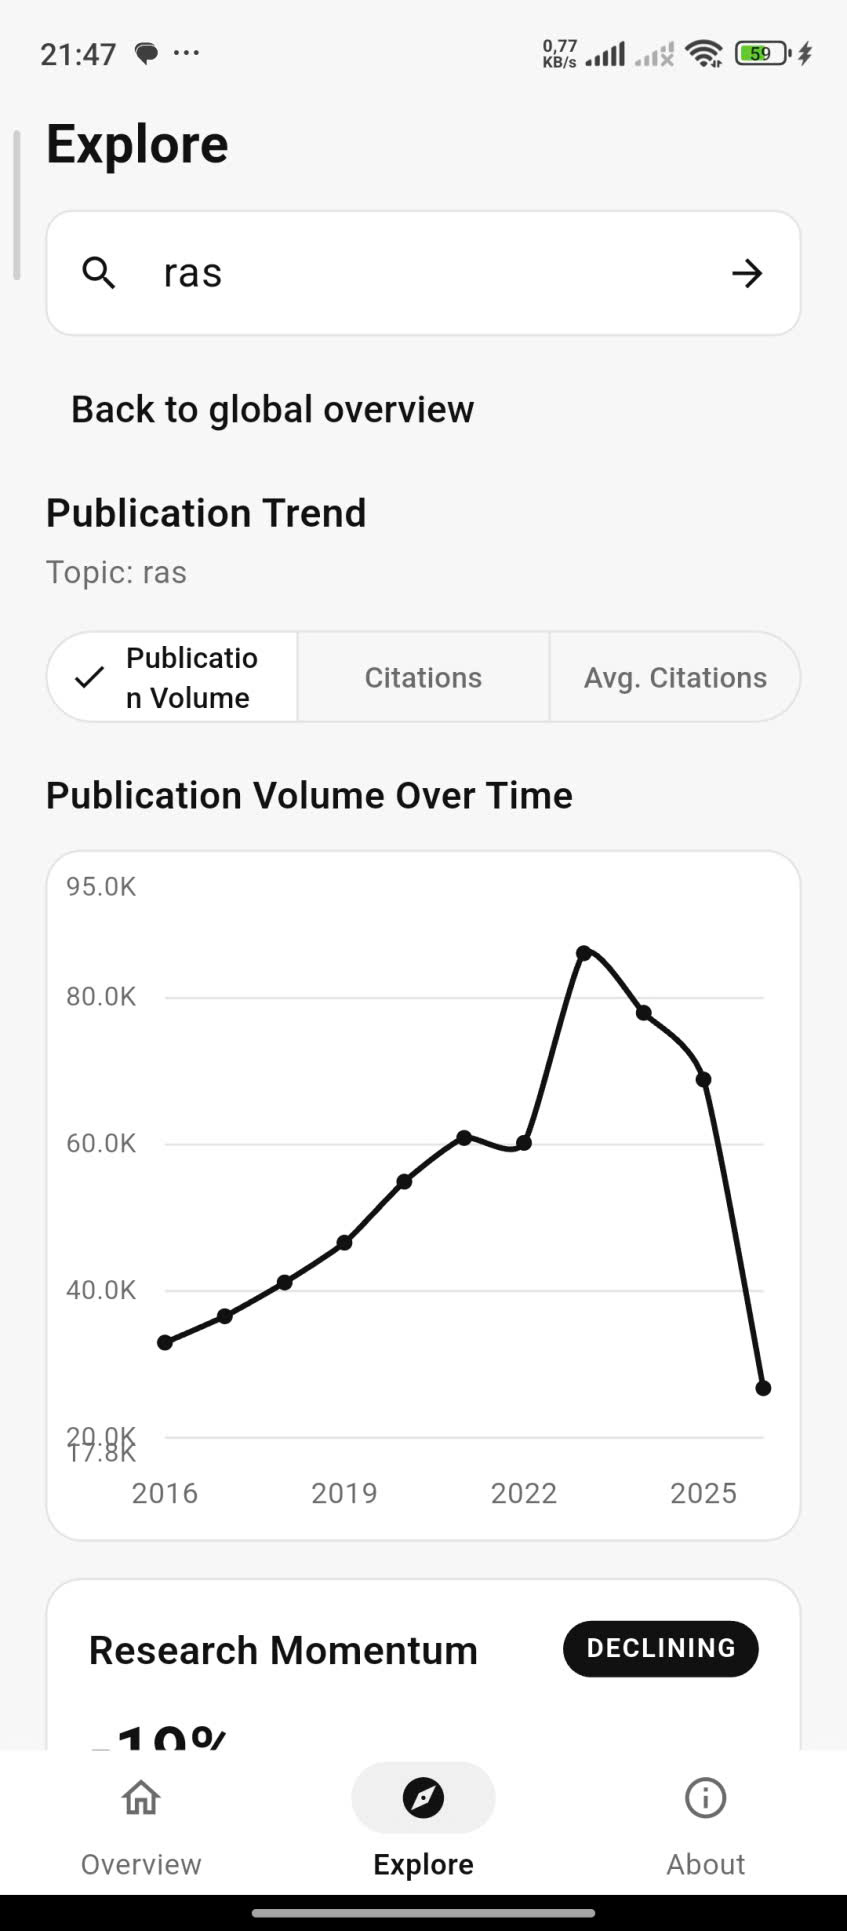
\includegraphics[width=\textwidth]{fig04-explore-trend.jpg}
    \caption{Line chart — publication volume by year}
  \end{subfigure}\hfill
  \begin{subfigure}{0.48\textwidth}
    \centering
    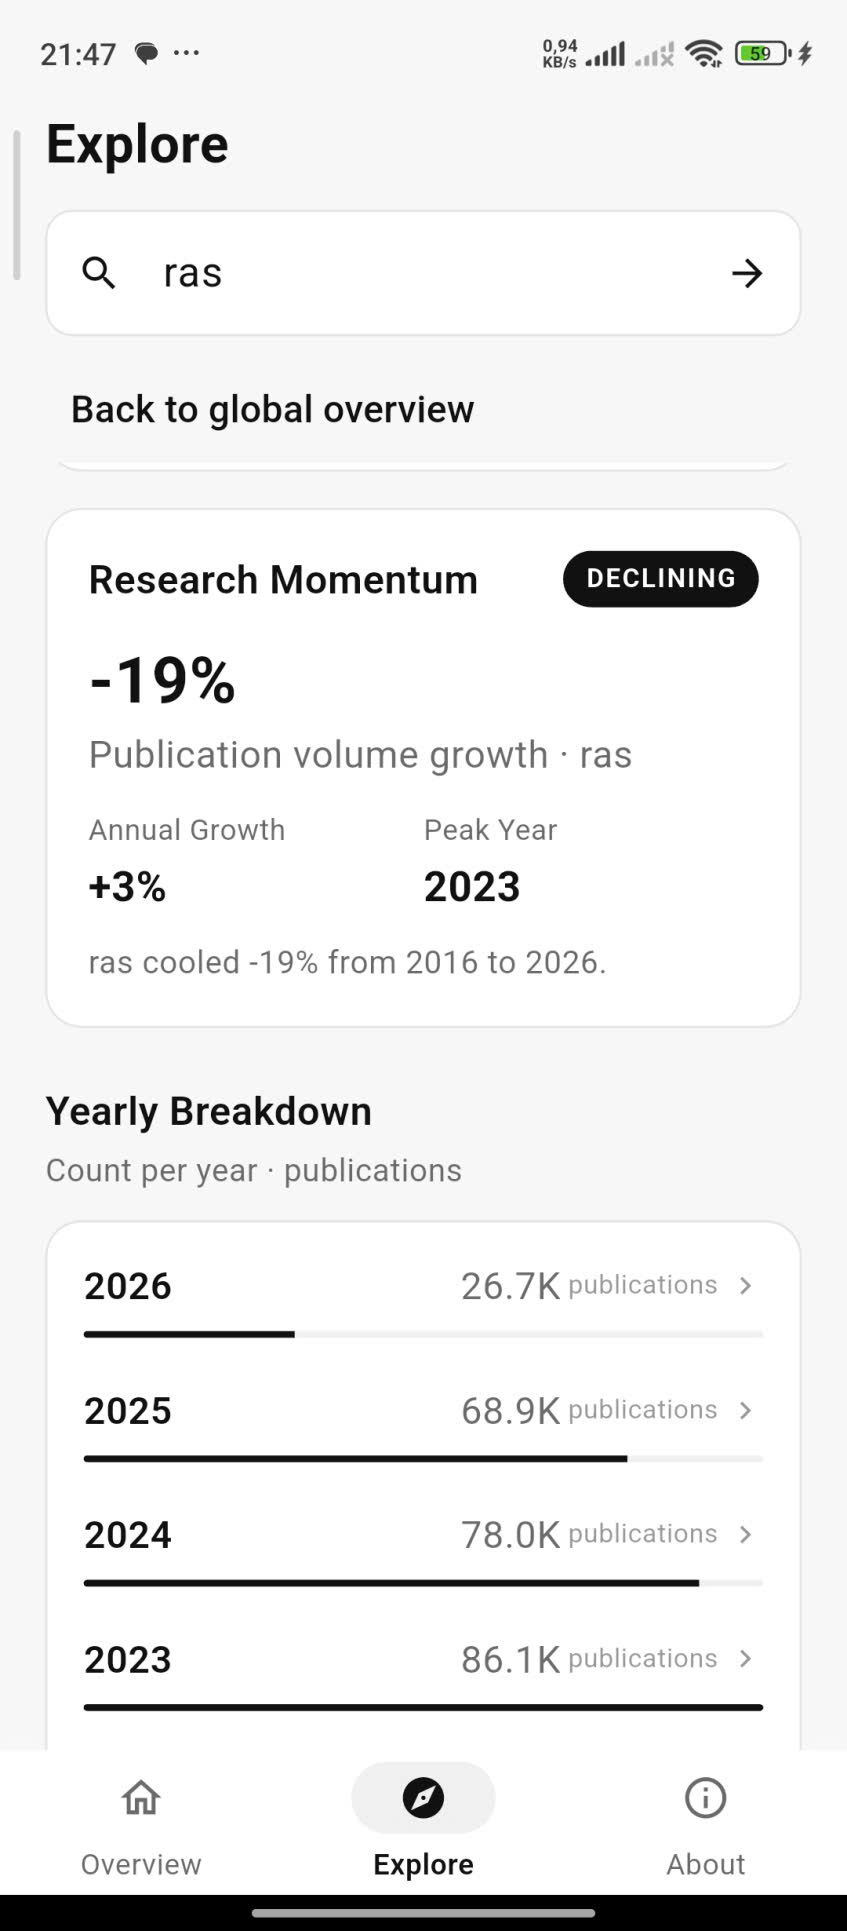
\includegraphics[width=\textwidth]{fig05-explore-momentum.jpg}
    \caption{Growth momentum and yearly breakdown}
  \end{subfigure}
  \caption{Trend analysis results after search}
\end{figure}

\begin{figure}[htbp]
  \centering
  
\includegraphics[width=0.42\textwidth]{fig06-explore-papers.jpg}
  \caption{Publication list sorted by citation count}
\end{figure}

\subsection{Publication Detail (Section 4.2)}
\begin{figure}[htbp]
  \centering
  
\includegraphics[width=0.42\textwidth]{fig07-detail.jpg}
  \caption{Publication details: title, authors, abstract, and citation count}
\end{figure}

\subsection{Journal and Author Detail}
\begin{figure}[htbp]
  \centering
  \begin{subfigure}{0.48\textwidth}
    \centering
    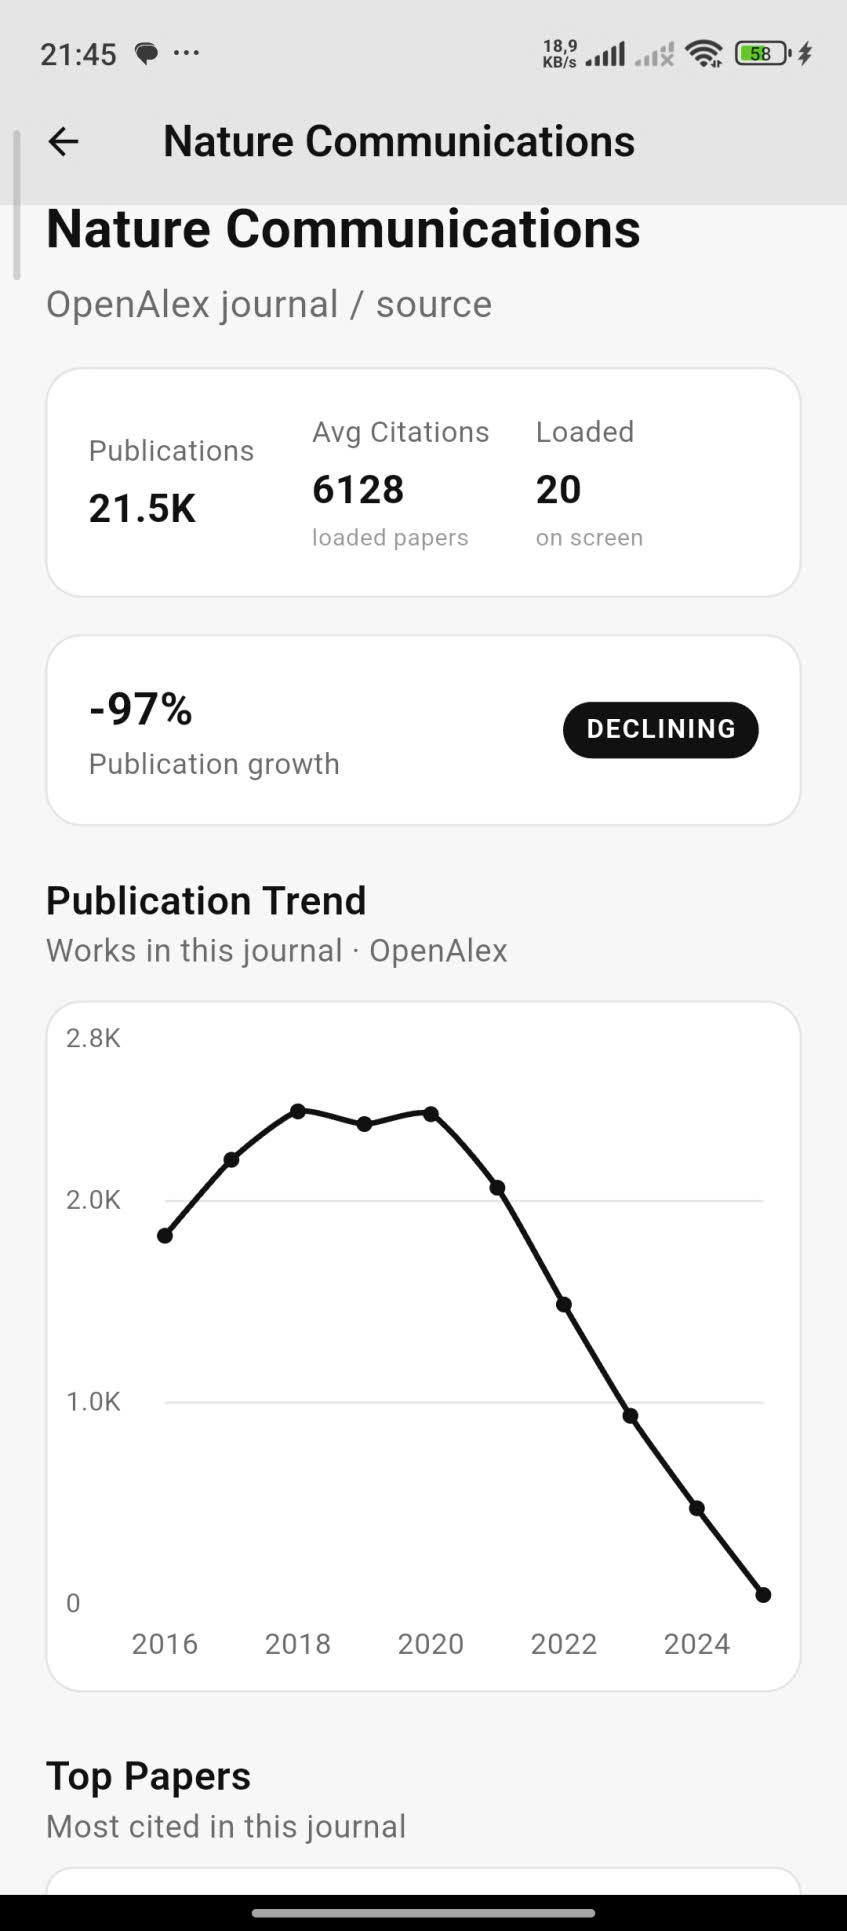
\includegraphics[width=\textwidth]{fig09-journal-trend.jpg}
    \caption{Journal detail with trend chart}
  \end{subfigure}\hfill
  \begin{subfigure}{0.48\textwidth}
    \centering
    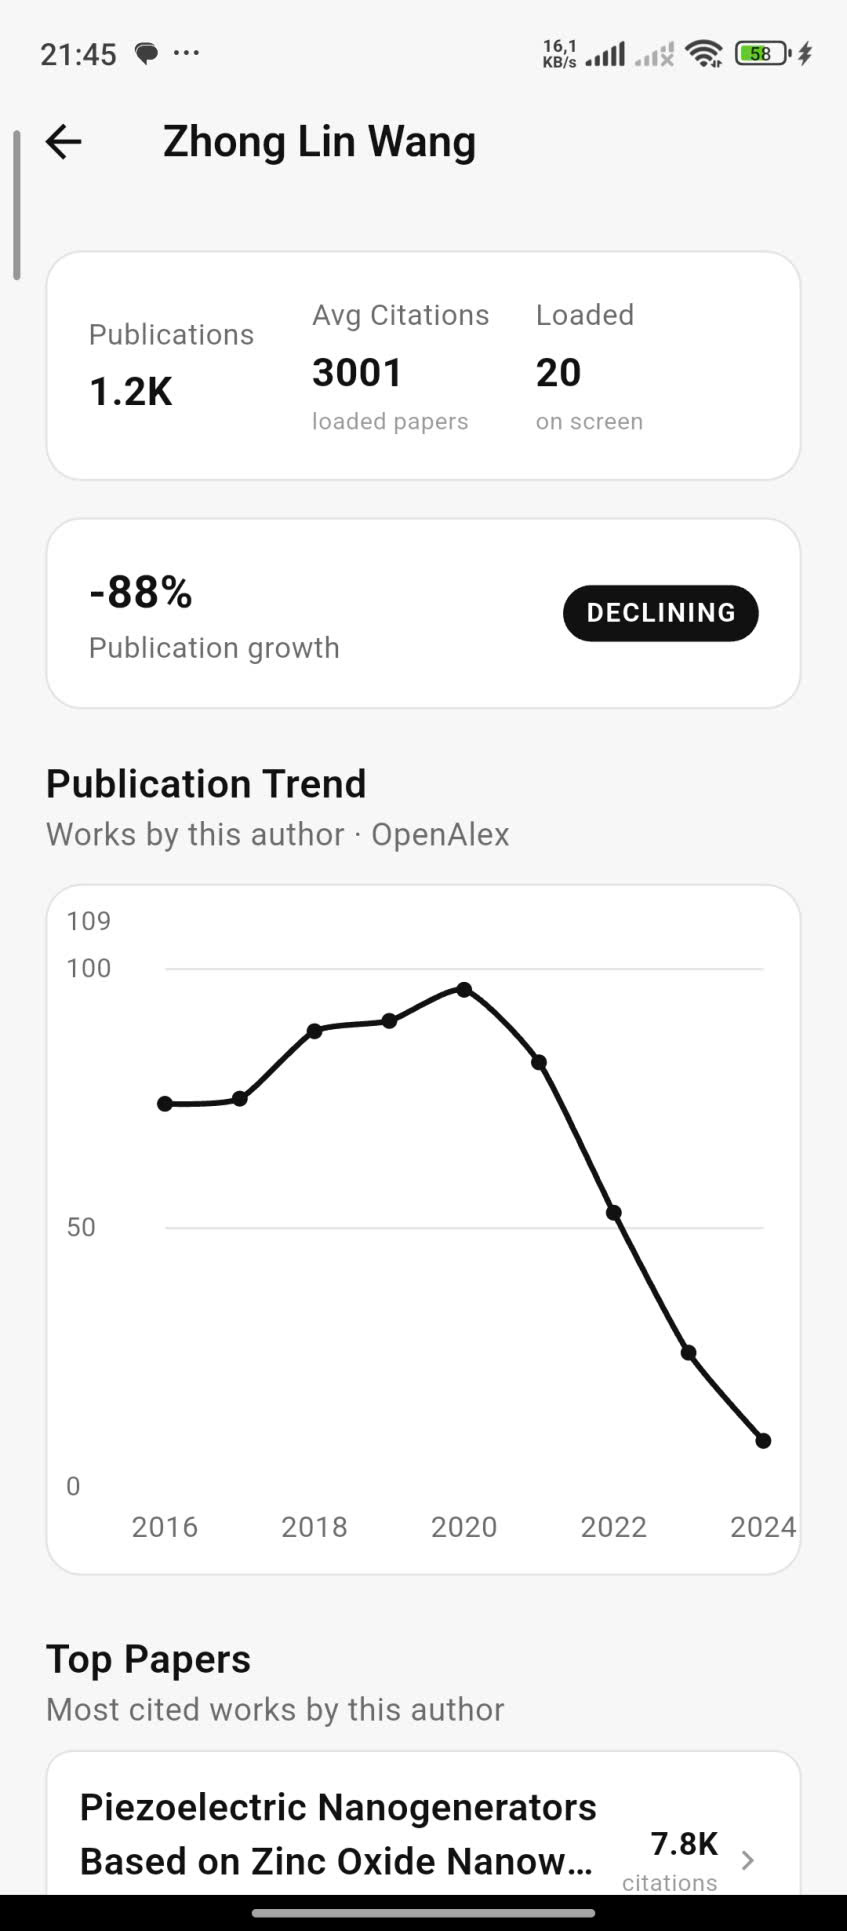
\includegraphics[width=\textwidth]{fig10-author-trend.jpg}
    \caption{Author detail with trend chart}
  \end{subfigure}
  \caption{Detail screens accessed from the dashboard or search results}
\end{figure}

\subsection{About Tab}
\begin{figure}[htbp]
  \centering
  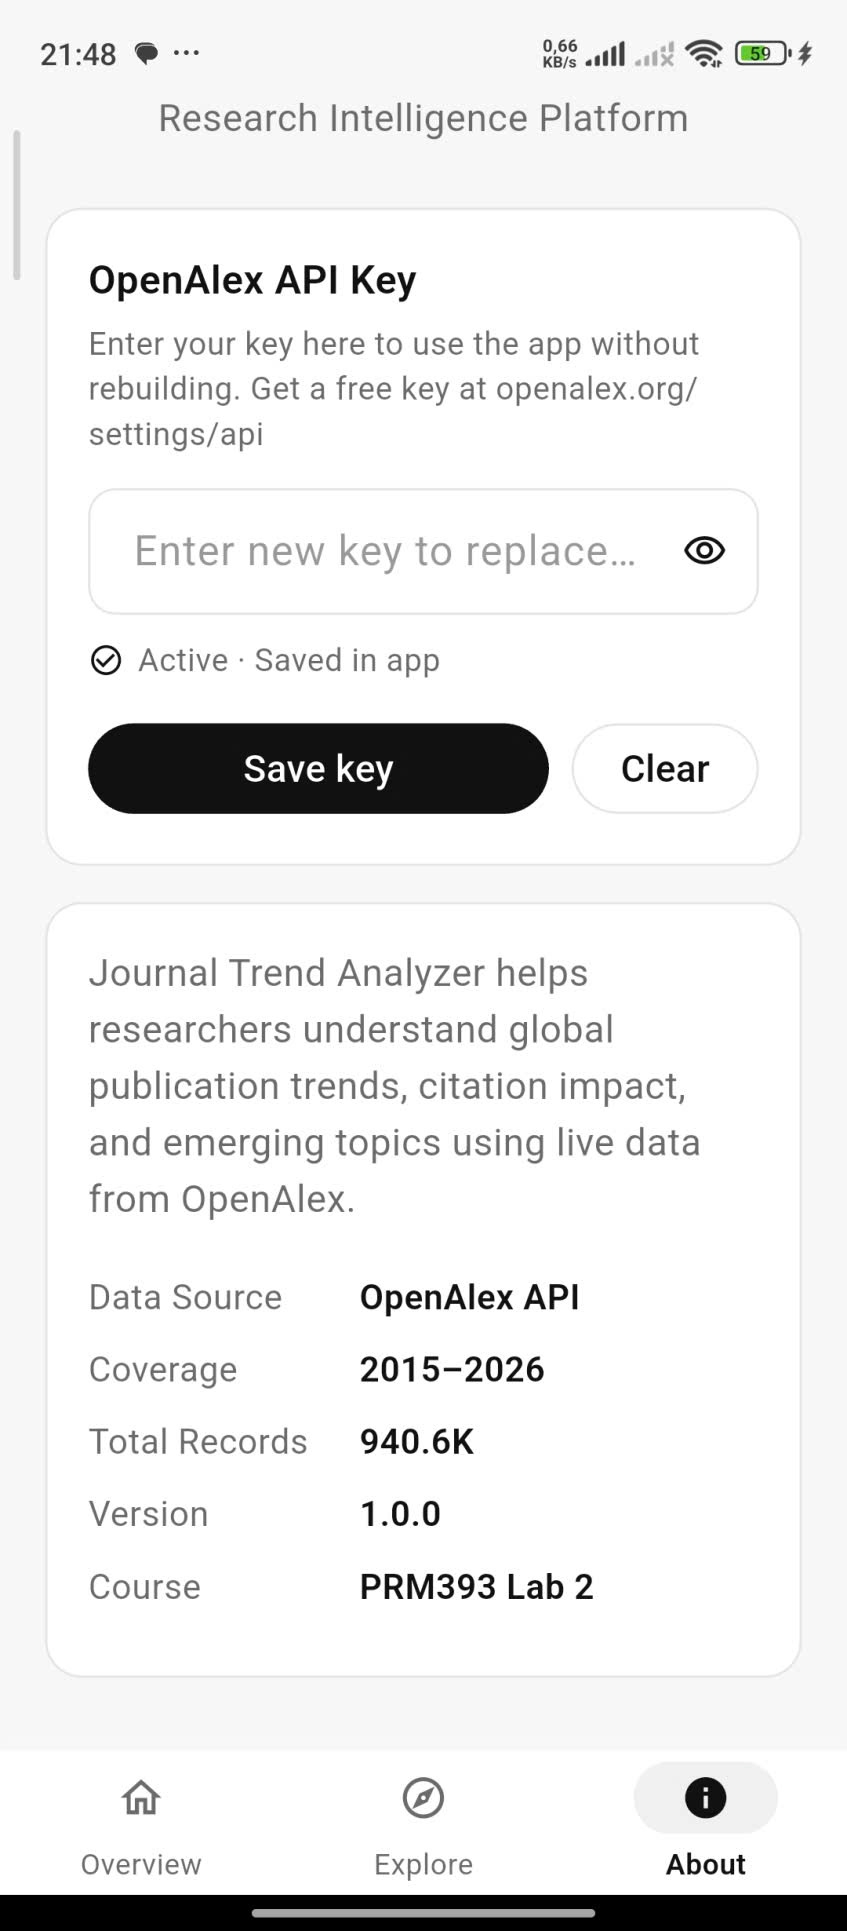
\includegraphics[width=0.42\textwidth]{fig08-about.jpg}
  \caption{Application information and OpenAlex API configuration}
\end{figure}

\end{document}
